%
% File: chap07.tex
% Author: Nadeem Gul Rintu Daniel
% Description: Gives an Overview of the implemented System with Screenshots
%
\let\textcircled=\pgftextcircled
\chapter{Floe Navigation App Overview}
\label{chap:fnsoverview}
\noindent
\initial{T}his section gives a brief description of the implemented Floe Navigation System. It will show how the Navigation System described in Chapter 6 is implemented and how the system looks like from the perspective of a User and Administrator. The Floe Navigation Android Application can be installed on any Android tablet. For detailed information, check the Floe Navigation User Guide and Floe Navigation Administrator Guide.%%Include Citation  
%
%=======
\section{User Menu}
\label{sec:sec7_1}
\noindent
 This section describes how to use the Floe Navigation Application. It provides a basic description of the menus in the App for the User. The screenshots shown here are based on the default product configuration.
%
\subsection{Dashboard}
\label{subsec:subsec7_1_1}
\noindent
The Dashboard is the main screen of the App. It is the first screen that the user sees after launching the app. Using the Dashboard, the user can navigate to all the sections of the app as shown in figure~\ref{fig:CH7MainDashboard}.
%
% A single figure
\begin{figure}[h]
	\centering
	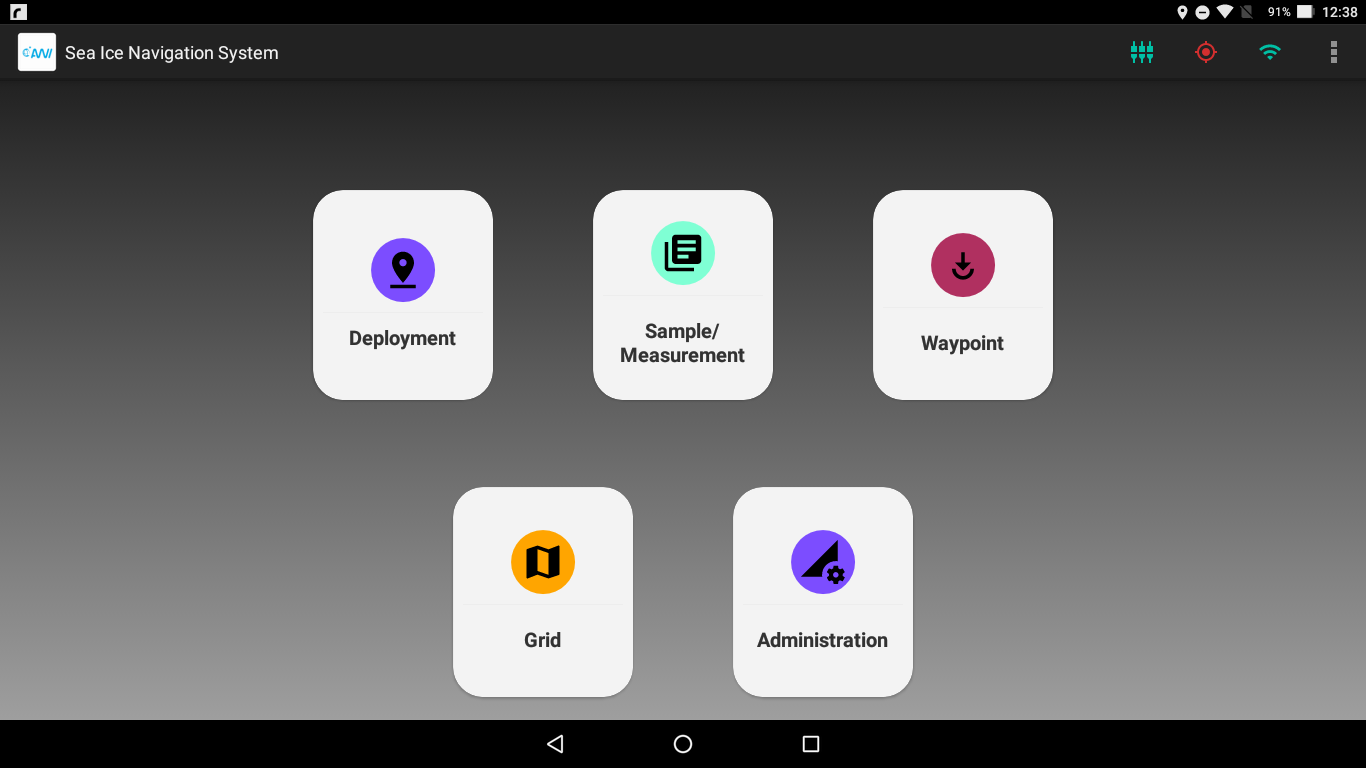
\includegraphics[height=0.3\textheight]{fig07/MainDashboard}
	\mycaption[Dashboard as seen on Android Tablet.]{Dashboard as seen on Android Tablet. }
	\label{fig:CH7MainDashboard}
\end{figure}
\newline
\noindent
The following icons are visible on the Dashboard:
\begin{itemize}
	\item \textbf{Deployment:} Can be used to deploy a static station. 
	\item \textbf{Sample/Measurement:} To take a Sample/Measurement on the Ice.
	\item \textbf{Waypoint:} Insert a waypoint on the Grid. 
	\item \textbf{Grid:} Show a visual representation of the whole coordinate system.
	\item \textbf{Administrator:} For the administration of the App. 
\end{itemize}
%
\subsection{Grid}
\label{subsec:subsec7_1_2}
\noindent
The Grid is a visual representation of the coordinate system established on the sea ice. As shown in figure~\ref{fig:CH7GridwithLayers}, the Grid shows all the stations and points of interest in a 100 km radius from the origin.
%
\begin{figure}[h]
	\centering
	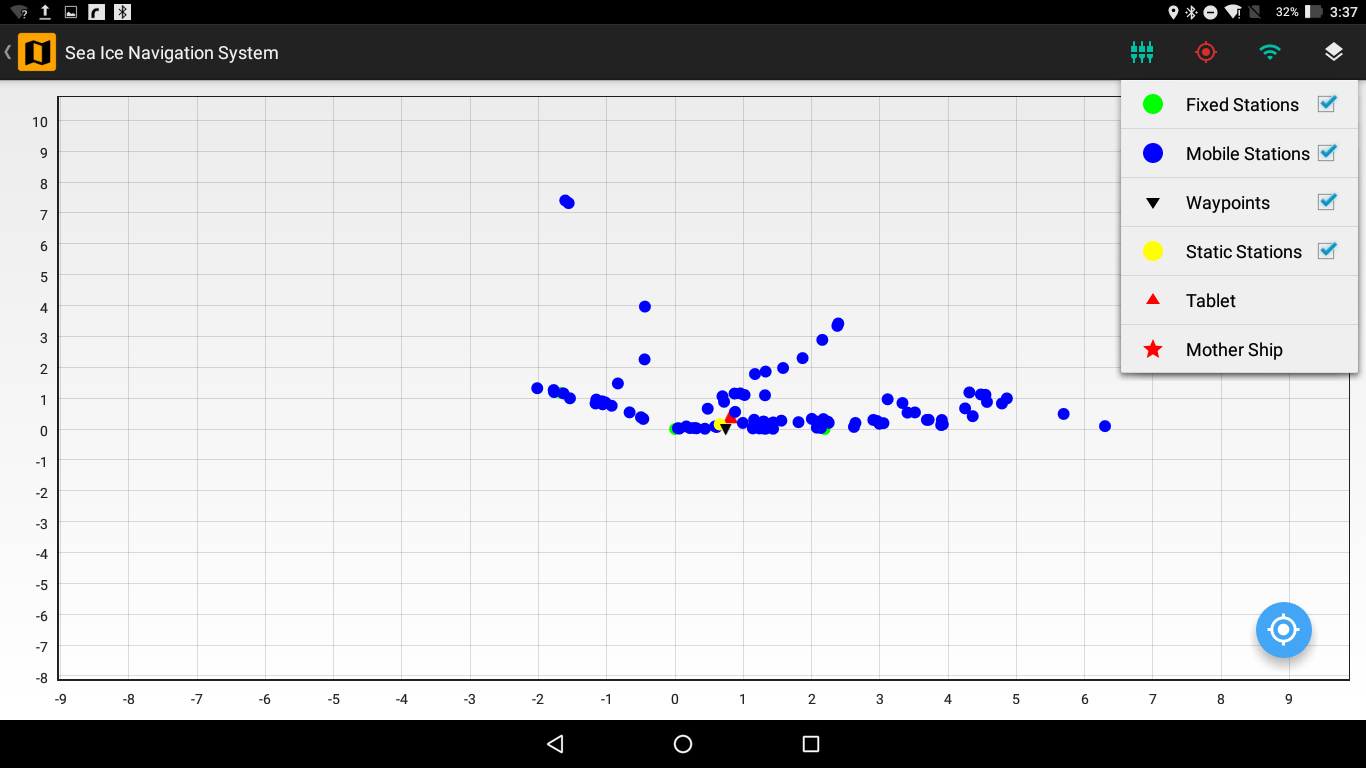
\includegraphics[height=0.3\textheight]{fig07/GridwithLayers.png}
	\mycaption[Visual Representation of the Coordinate System.]{Visual Representation of the Coordinate System. }
	\label{fig:CH7GridwithLayers}
\end{figure}
%
\newpage
\noindent
Table~\ref{tbl:CH7gridLayers} shows the layers that are visible on the Grid by default along with their respective icons.
%
\begin{table}[h]
	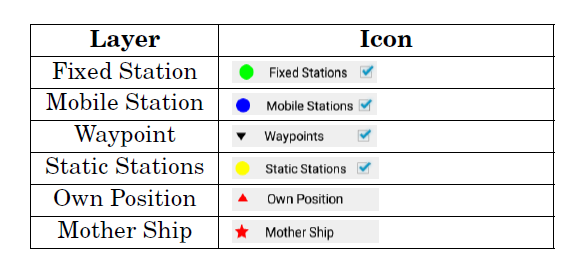
\includegraphics[width=0.75\linewidth]{fig07/LayerTable.png}
	\centering
	\mycaption[Available Layers in Grid.]{Available Layers in Grid.}
	\label{tbl:CH7gridLayers}
\end{table}
%
\newline
\noindent
Tapping the icon of a station shows the relevant details of that station as shown in figure~\ref{fig:CH7GridwithBox}.
\begin{figure}[h]
	\centering
	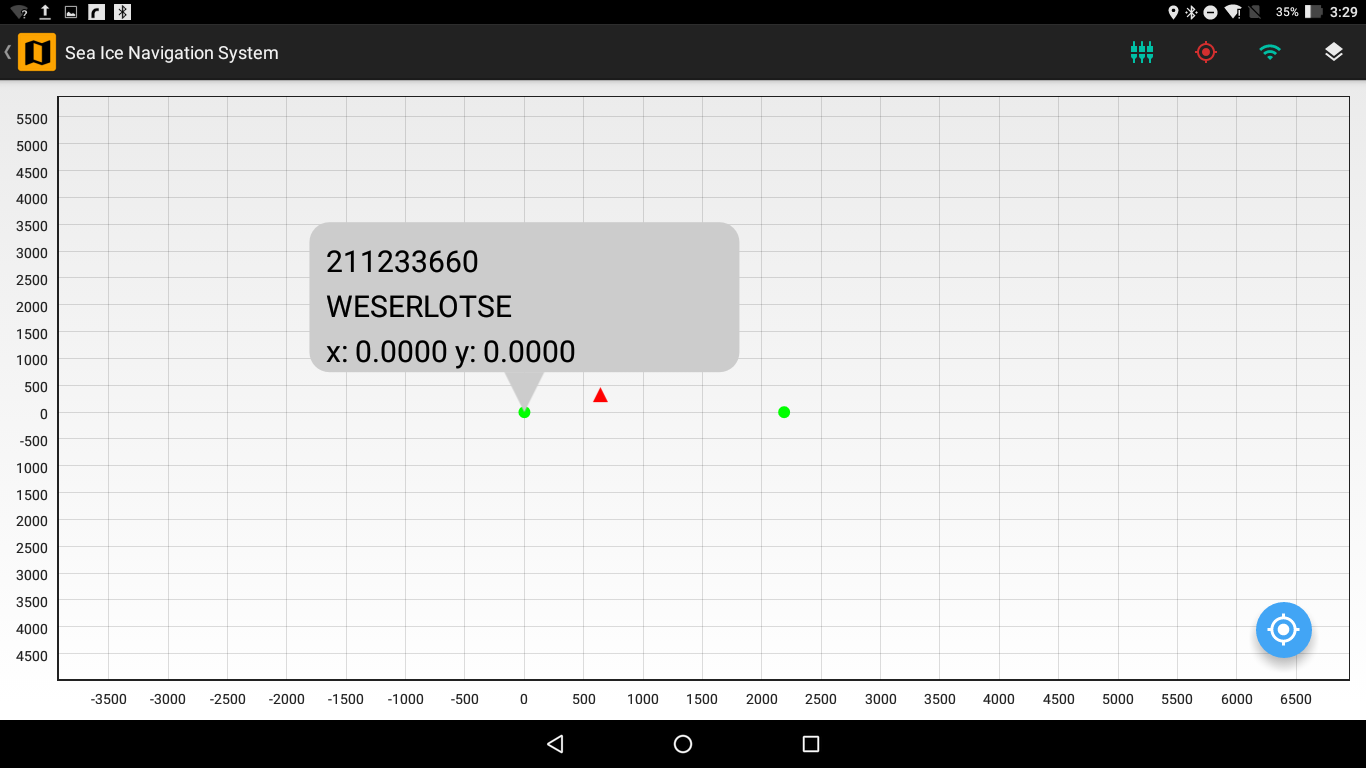
\includegraphics[height=0.3\textheight]{fig07/GridwithBox.png}
	\mycaption[Details Box for a Station.]{Details Box for a Station.}
	\label{fig:CH7GridwithBox}
\end{figure}
%
\subsection{Deployment}
\label{subsec:subsec7_1_3}
\noindent
As described in Chapter \textbf{(give reference here)} Static Stations are fixed points on the Sea Ice where any equipment or structure has been installed without an AIS Transponder. You can install a new Static Station by tapping on the Deployment button on the Main Dashboard which opens the Deployment screen. Static Stations once installed can only be deleted by an administrator. Figure~\ref{fig:CH7StaticStationDeployment} shows the Deployment screen.
%
\begin{figure}[h]
	\centering
	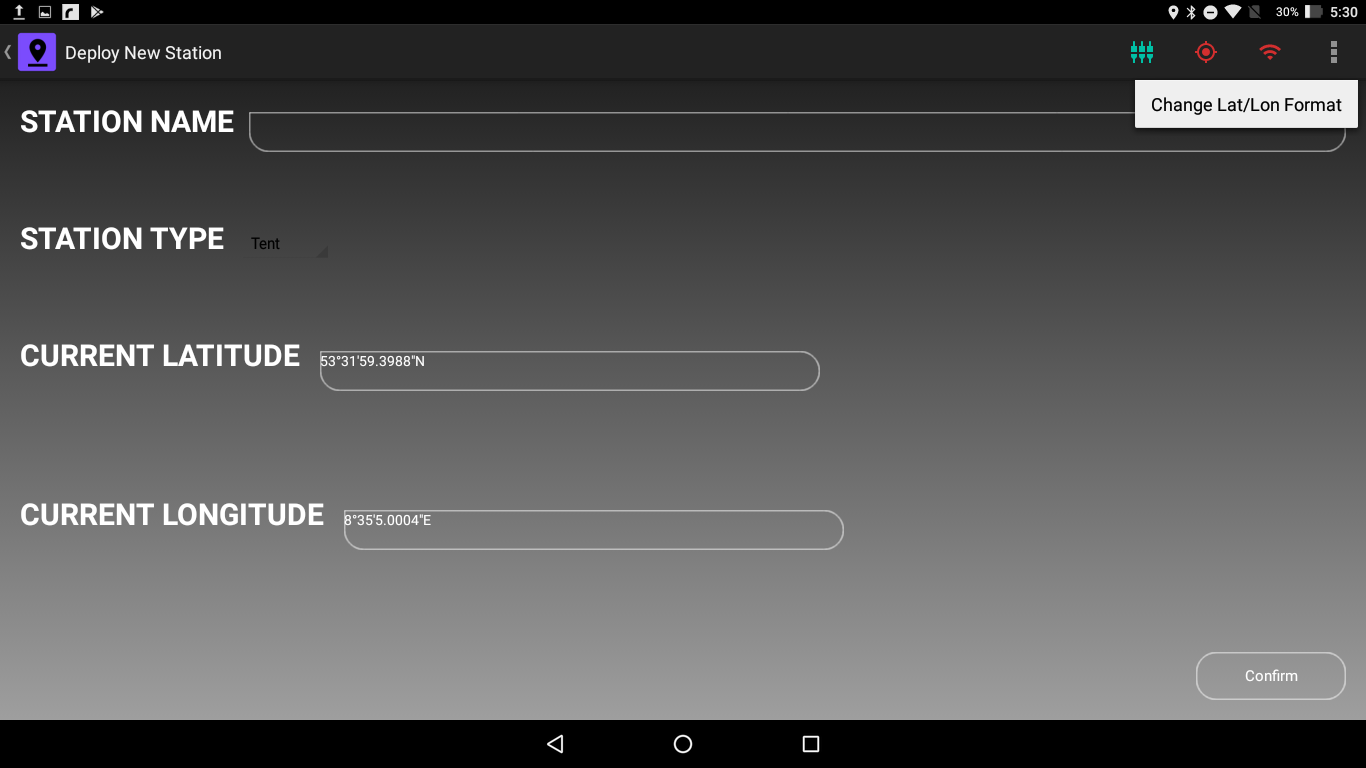
\includegraphics[height=0.3\textheight]{fig07/StaticStationDeployment.png}
	\mycaption[Deployment of a Static Station.]{Deployment of a Static Station.}
	\label{fig:CH7StaticStationDeployment}
\end{figure}
%
\subsection{Waypoint}
\label{subsec:subsec7_1_4}
\noindent
As described in Chapter \textbf{(give reference here)}, Waypoints are marked points of interest on the Sea Ice. Waypoints can be used to specify points along a track on the ice, or a single point where measurement can be taken in the future or it can also be used to marked danger zones or sensitive spots on the ice. Waypoints do not have an AIS data and hence are not used by the App to maintain the coordinate system.You can install a new Waypoint by tapping on the Waypoint button on the Main Dashboard which opens the Waypoint screen. Each Waypoint is identified by a unique label. Figure~\ref{fig:CH7Waypoint} shows the Waypoint installation screen.
%
\begin{figure}[h]
	\centering
	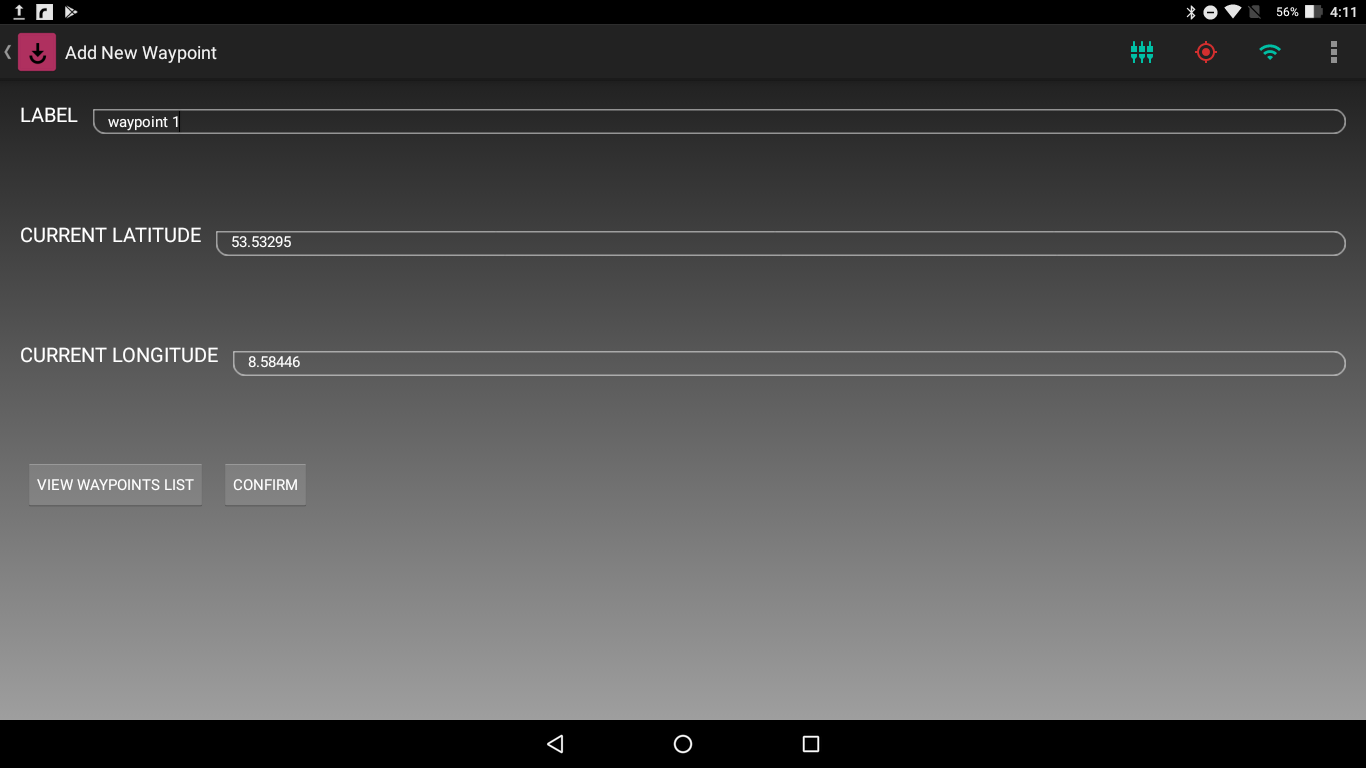
\includegraphics[height=0.3\textheight]{fig07/Waypoint.png}
	\mycaption[Installation of a Waypoint.]{Installation of a Waypoint.}
	\label{fig:CH7Waypoint}
\end{figure}
%
%\newpage
\subsection{Sample/Measurement}
\label{subsec:subsec7_1_5}
\noindent
\textbf{\textcolor{red}{Add Description after name and screenshots are updated}}.
As described in Chapter \textbf{(give reference here)}, Waypoints are marked points of interest on the Sea Ice. Waypoints can be used to specify points along a track on the ice, or a single point where measurement can be taken in the future or it can also be used to marked danger zones or sensitive spots on the ice. Waypoints do not have an AIS data and hence are not used by the App to maintain the coordinate system.You can install a new Waypoint by tapping on the Waypoint button on the Main Dashboard which opens the Waypoint screen. Each Waypoint is identified by a unique label. Figure~\ref{fig:CH7Sample} shows the Waypoint installation screen.
\begin{figure}[h]
	\centering
	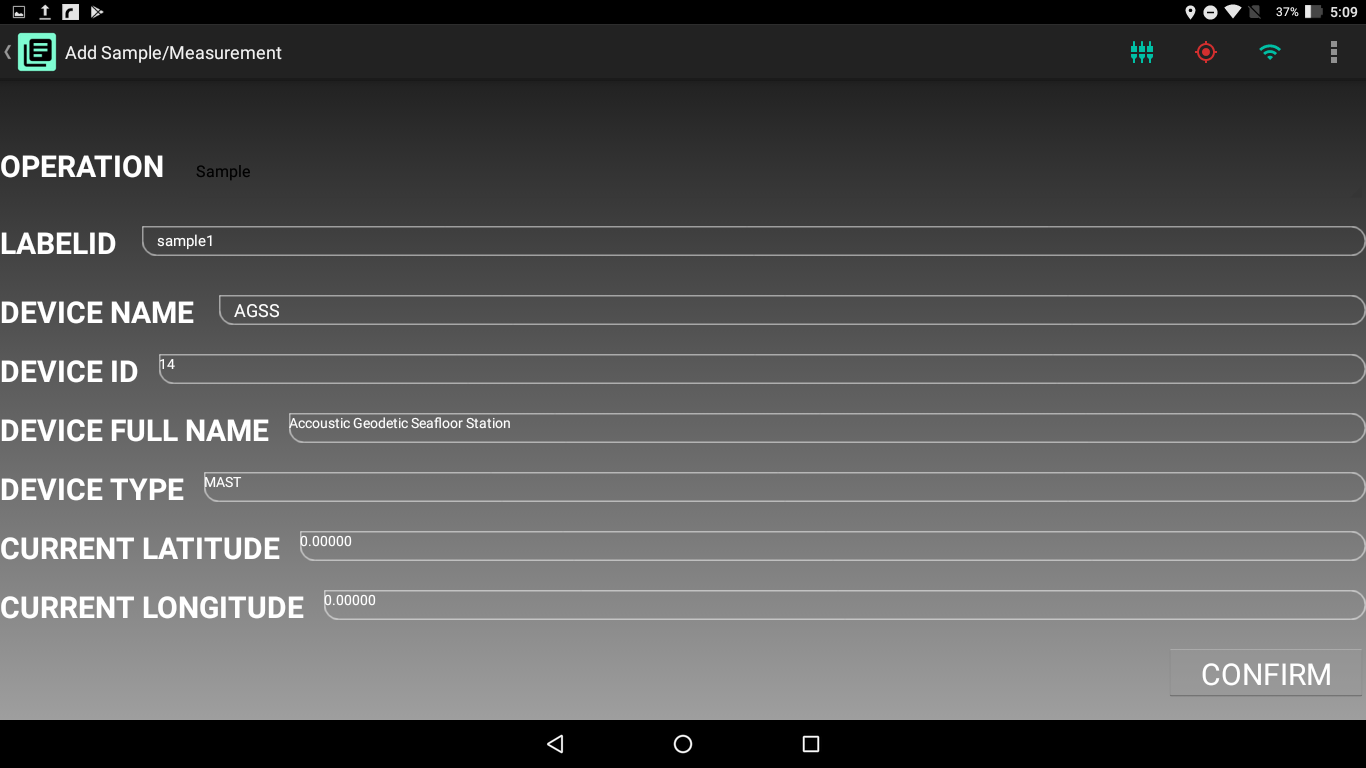
\includegraphics[height=0.3\textheight]{fig07/Sample.png}
	\mycaption[Installation of a Waypoint.]{Installation of a Waypoint.}
	\label{fig:CH7Sample}
\end{figure}
%
%\newpage
\section{Admin Menu}
\label{subsec:subsec7_2}
\noindent
This section describes how to administer the Floe Navigation Application. It provides a basic description of the menus in the App for the Administrator.
 
\subsection{Admin Dashboard}
\label{subsec:subsec7_2_1}
\noindent
The Admin Dashboard can be opened from the Main Dashboard of the Floe Navigation App. The Admin Dashboard can only be accessed with valid user credentials and it can be used to setup the coordinate system, synchronization and other admin tasks. Figure~\ref{fig:CH7AdminMenu} shows the Admin Dashboard.
\begin{figure}[h]
	\centering
	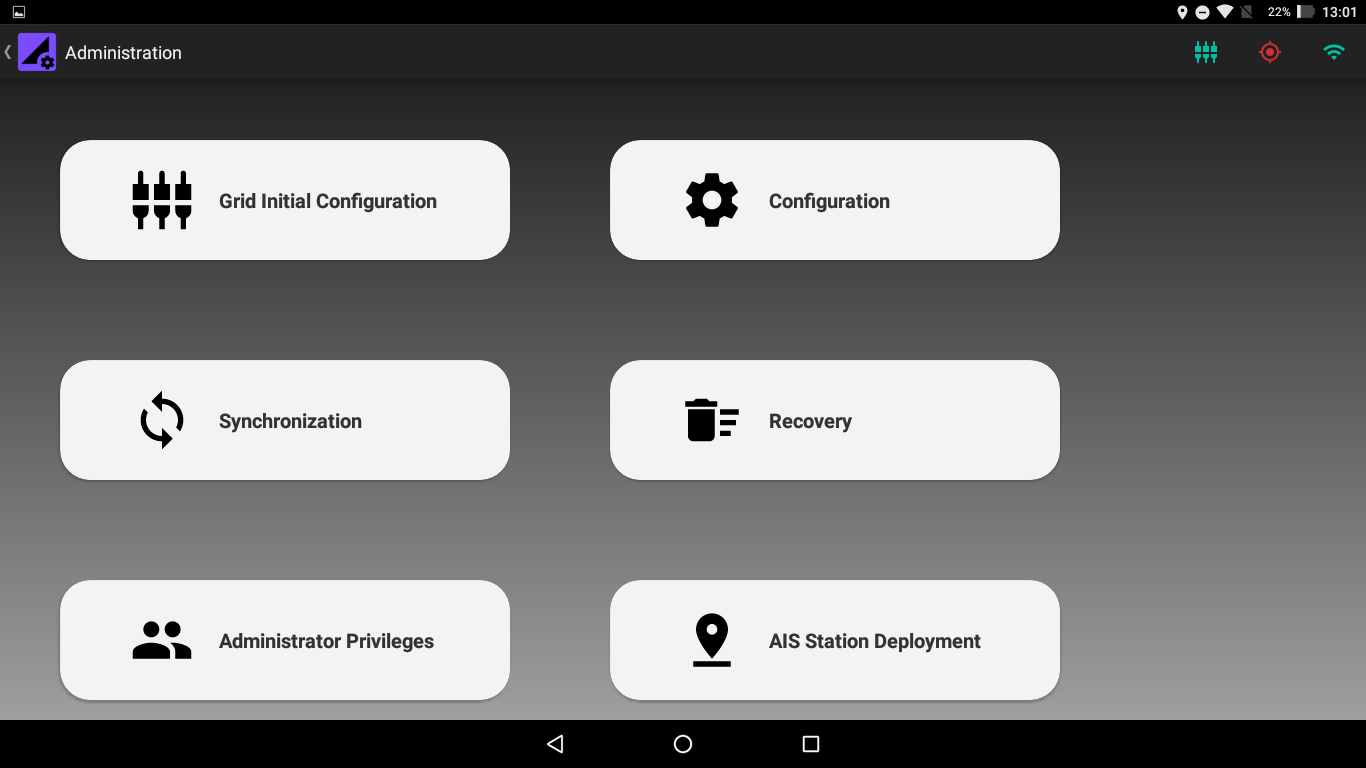
\includegraphics[height=0.3\textheight]{fig07/AdminMenu.png}
	\mycaption[Admin Dashboard.]{Admin Dashboard.}
	\label{fig:CH7AdminMenu}
\end{figure}
%
\newpage
\subsection{Grid Initial Configuration}
\label{subsec:subsec7_2_2}
\noindent
As described in Chapter \textbf{Insert Chapter Label here} the Floe Navigation system needs at least two AIS Transponders installed as Fixed Stations on the Sea Ice to create its coordinate system. The Admin needs to install two Fixed Stations to run the Configuration setup. The setup runs for a specified time and creates a coordinate system when finished. Figure~\ref{fig:CH7SetupScreen} shows a configuration setup in progress. 
\begin{figure}[h]
	\centering
	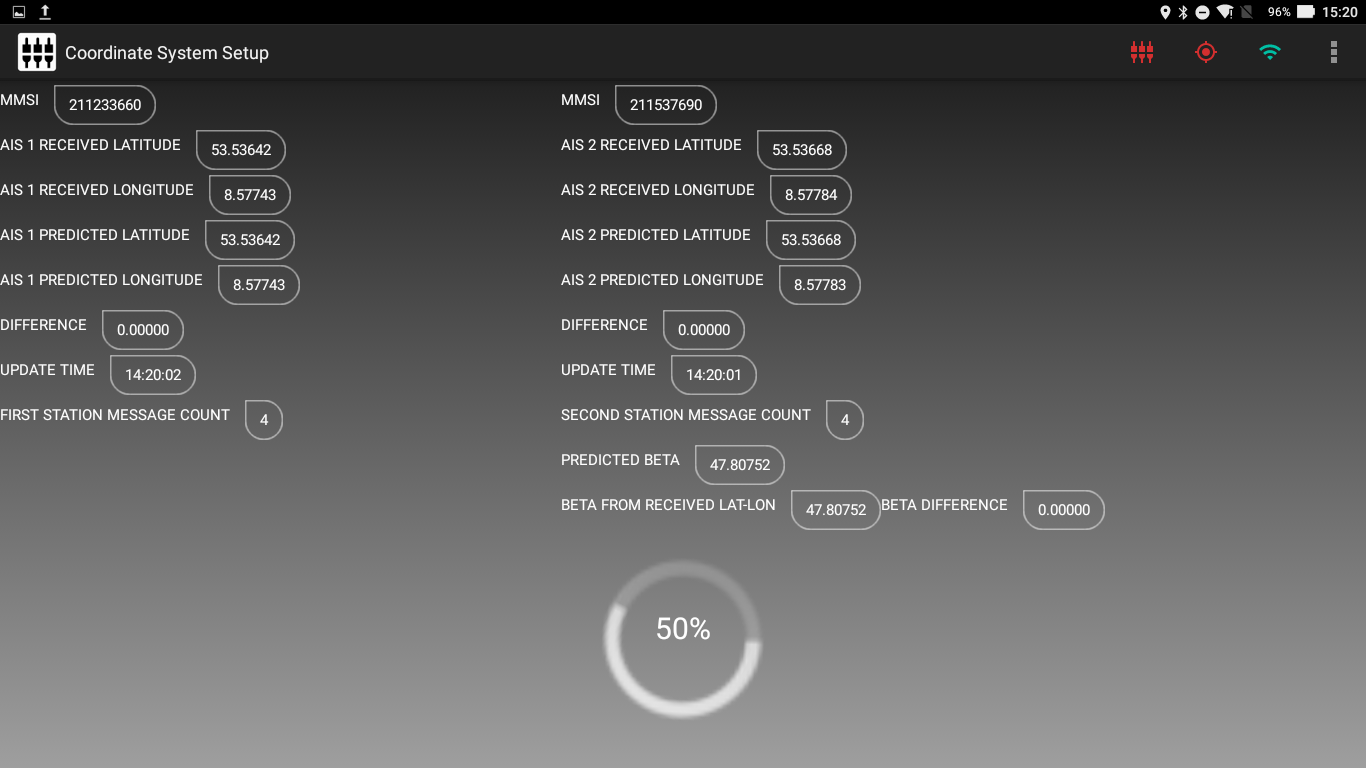
\includegraphics[height=0.3\textheight]{fig07/SetupScreen.png}
	\mycaption[Grid Initial Configuration in progress.]{Grid Initial Configuration in progress.}
	\label{fig:CH7SetupScreen}
\end{figure}
%
\subsection{Configuration}
\label{subsec:subsec7_2_3}
\noindent
Certain important parameters can be configured by the admin which are used by the App for its background services and this can be done using the Configuration menu. Figure~\ref{fig:CH7ConfigParams} shows the configuration parameters. 
\begin{figure}[h]
	\centering
	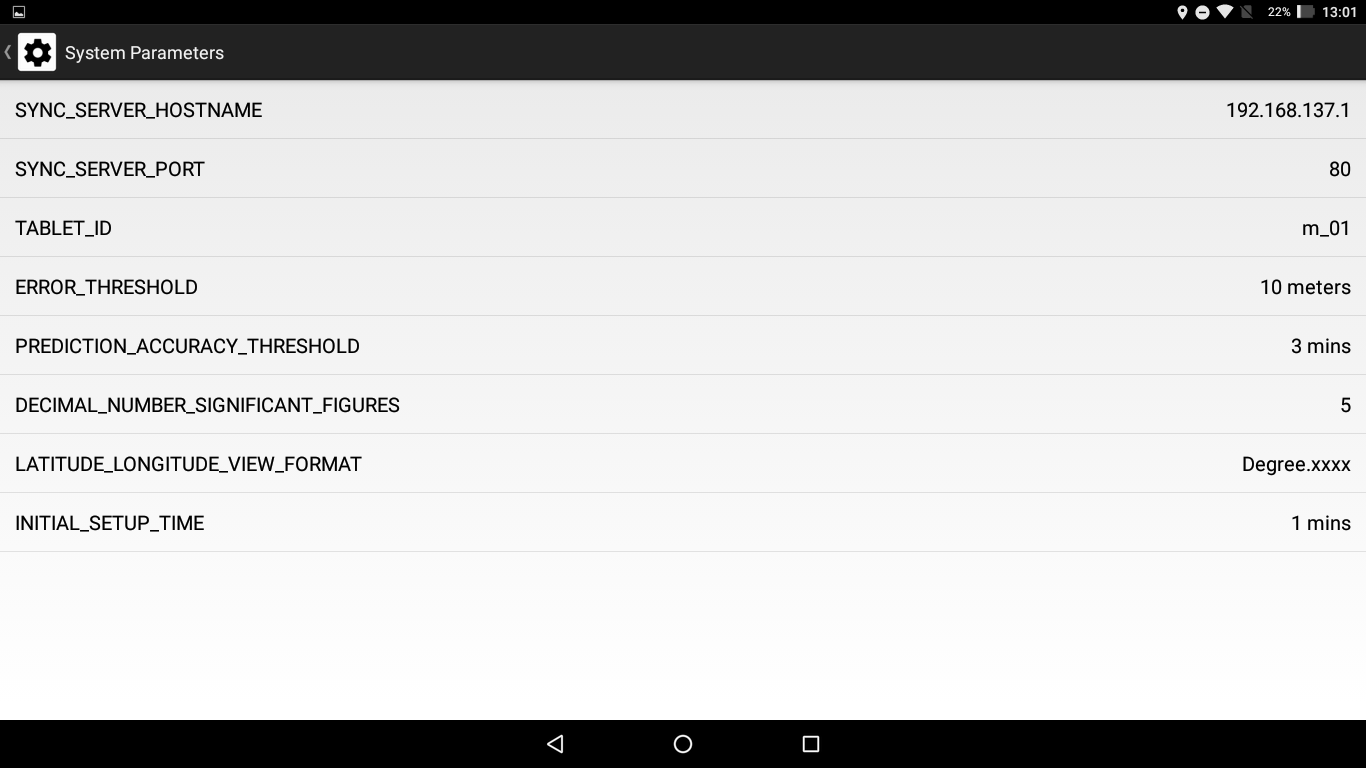
\includegraphics[height=0.3\textheight]{fig07/ConfigParameters.png}
	\mycaption[List of Configurable Parameters.]{List of Configurable Parameters.}
	\label{fig:CH7ConfigParams}
\end{figure}
%
\subsection{Synchronization}
\label{subsec:subsec7_2_4}
\noindent
Synchronization process ensures that all the important data which is used to create and maintain the coordinate system remains the same in all the tablets. When the coordinate system has been established on one tablet; that tablet must be synchronized with the Sync Server and the data is pulled into other tablets to set up the coordinate system. This helps in maintaining a uniform coordinate system in all the tablets. The Device list which is used to take Sample/Measurement is also imported with the Synchronization process. Figure~\ref{fig:CH7SyncScreen} shows the synchronization tool on the App. 
\begin{figure}[h]
	\centering
	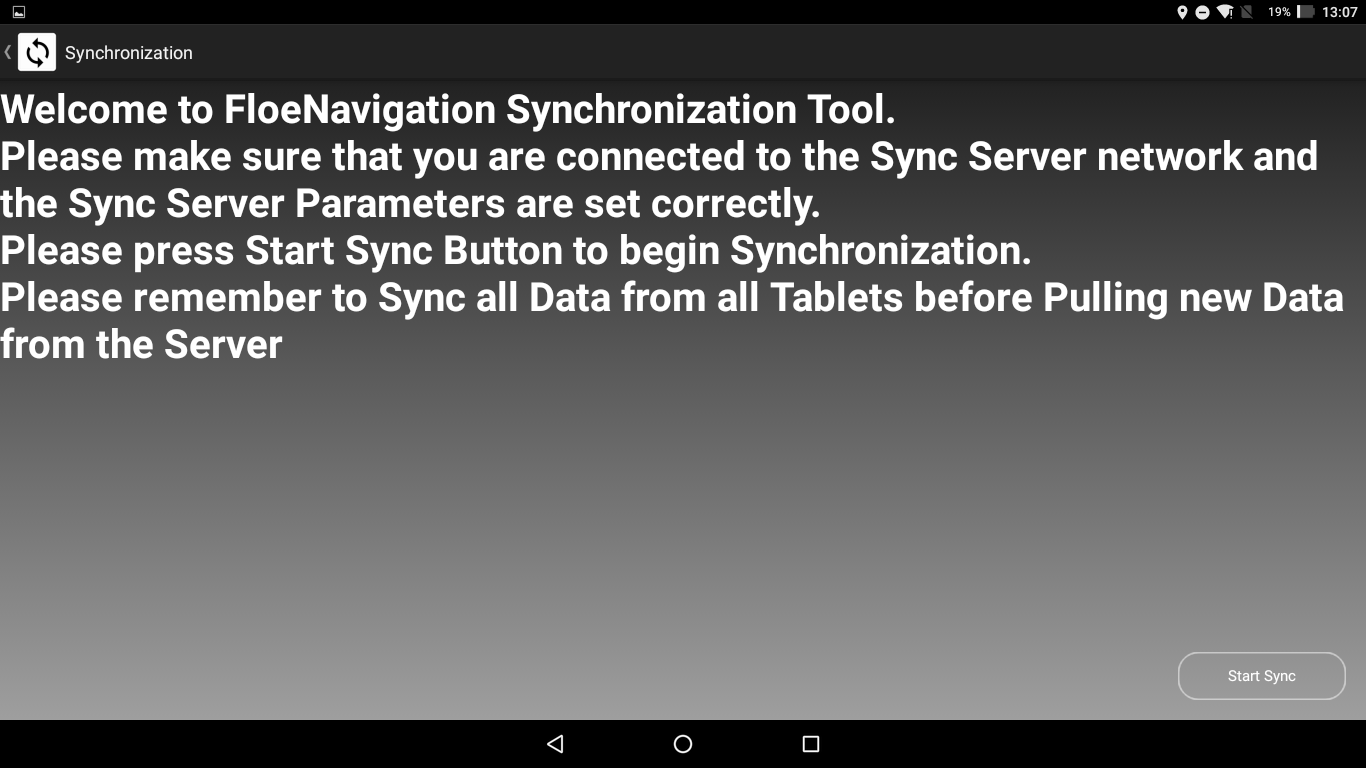
\includegraphics[height=0.3\textheight]{fig07/SyncScreen.png}
	\mycaption[Sync Tool.]{Synchronization Tool.}
	\label{fig:CH7SyncScreen}
\end{figure}
%\newpage
Figure~\ref{fig:CH7SyncInProgress} shows a running synchronization process. 
\begin{figure}[h]
	\centering
	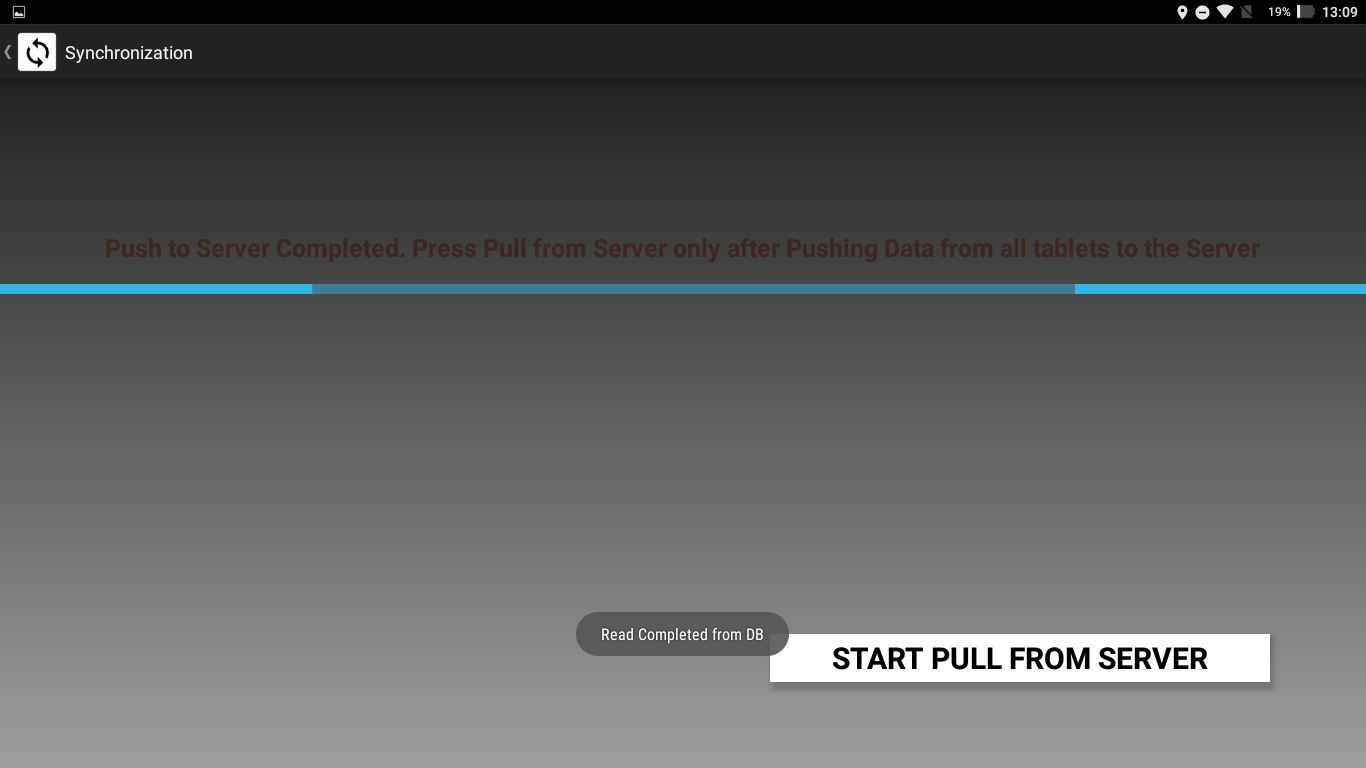
\includegraphics[height=0.3\textheight]{fig07/SyncInProgress.png}
	\mycaption[Synchronization in Progress.]{Synchronization in Progress.}
	\label{fig:CH7SyncInProgress}
\end{figure}
%
\newpage
\subsection{Recovery}
\label{subsec:subsec7_2_5}
\noindent
When a Fixed Station is no longer in use or if the Sea Ice breaks, the AIS Transponder on that position can be recovered and reused in another position. If a Fixed Station is recovered, it is no longer used to maintain the coordinate system by the app and the AIS transponder if it is powered on, will become a Mobile Station until it is reinstalled as a Fixed Station. Similarly, a Static Station can also be removed if it is no longer useful. Fixed Station and Static Stations can only be recovered by an Administrator of the Floe Navigation App.  Figure~\ref{fig:CH7Recovery} shows the recovery of a Fixed Station. 
\begin{figure}[h]
	\centering
	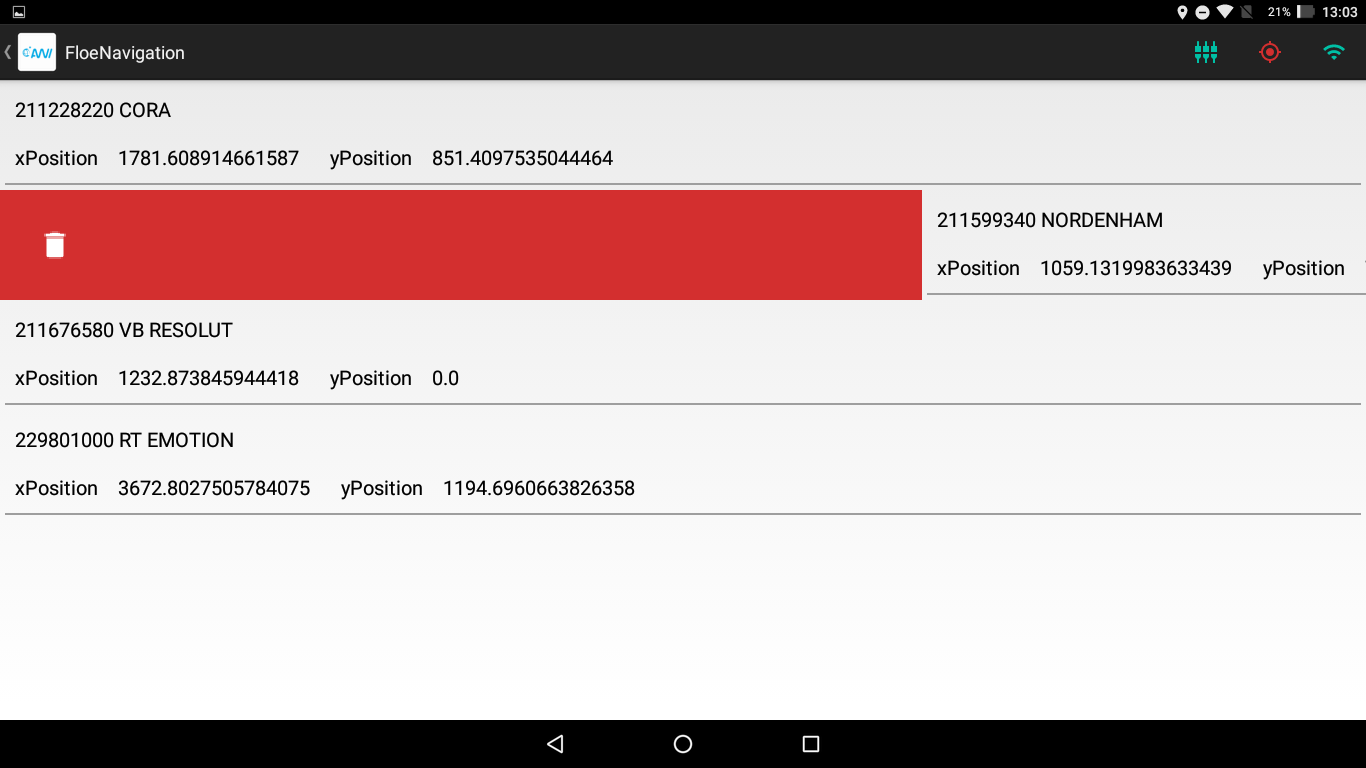
\includegraphics[height=0.3\textheight]{fig07/Recovery.png}
	\mycaption[Recovery of a Station.]{Recovery of a Station.}
	\label{fig:CH7Recovery}
\end{figure}
%
\subsection{Administrator Privileges}
\label{subsec:subsec7_2_6}
\noindent
Administrators can be added or removed using the Administrator Privileges Menu. Figure~\ref{fig:CH7AdminPrivileges} shows the Administrator Privileges Menu. 
\begin{figure}[h]
	\centering
	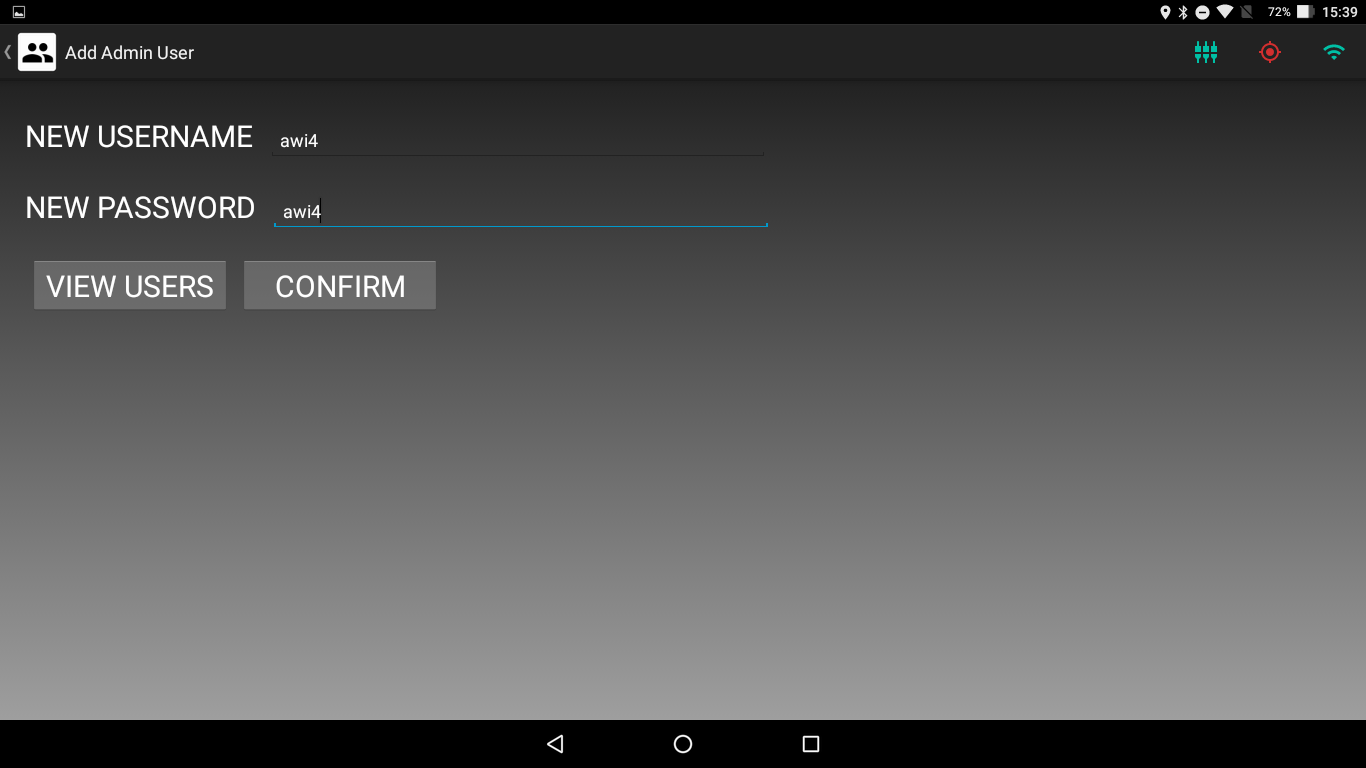
\includegraphics[height=0.3\textheight]{fig07/AdminPrivileges.png}
	\mycaption[Creating a New Administrator.]{Creating a New Administrator.}
	\label{fig:CH7AdminPrivileges}
\end{figure}
%\newpage
%
\subsection{AIS Station Deployment}
\label{subsec:subsec7_2_7}
\noindent
New Fixed Stations can be deployed by the Administrators. Figure~\ref{fig:CH7AISDeployment} shows the AIS Deployment Screen. 
\begin{figure}[h]
	\centering
	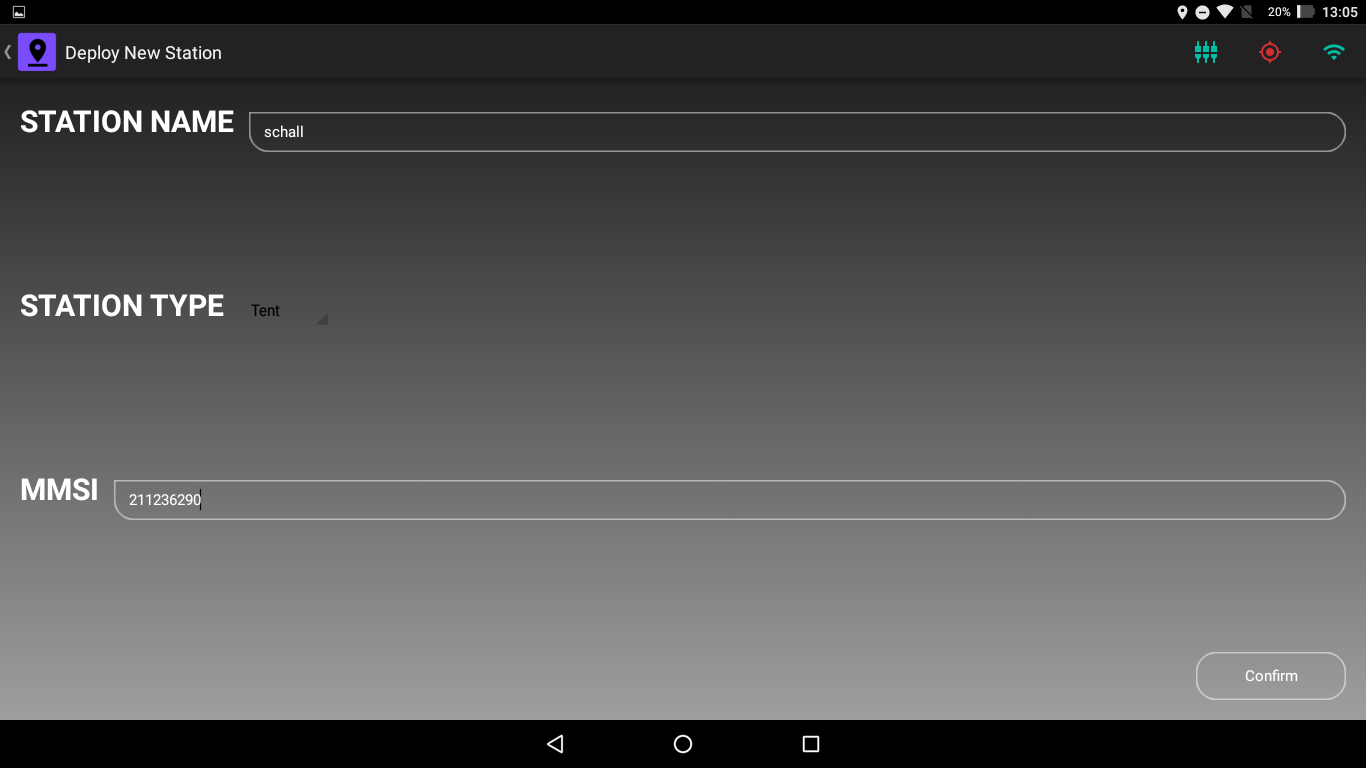
\includegraphics[height=0.3\textheight]{fig07/AISDeployment.png}
	\mycaption[Deploying a new Fixed Station.]{Deploying a new Fixed Station.}
	\label{fig:CH7AISDeployment}
\end{figure}
%
%=========================================================